\documentclass[12pt,a4paper,oneside]{report}
\usepackage[a4paper,left=35mm,right=25mm,top=25mm,bottom=25mm]{geometry}
\usepackage{amsmath,amssymb}
\usepackage{newtxtext,newtxmath}
\usepackage{setspace,graphicx,booktabs,tabularx,enumitem}
\usepackage{tikz}
\usetikzlibrary{positioning,arrows.meta}
\usepackage[numbers,sort&compress]{natbib}
\usepackage[hidelinks]{hyperref}
\usepackage{caption}
\usepackage{algorithm,algpseudocode,listings,xcolor}
\usepackage{fancyhdr}
\setlength{\headheight}{15pt}
\pagestyle{fancy}
\fancyhf{}
\fancyhead[L]{\small B.Tech Project Report}
\fancyhead[R]{\small NIT Calicut}
\fancyfoot[C]{\thepage}
\lstset{basicstyle=\ttfamily\small,breaklines=true,frame=single,numbers=left,numberstyle=\tiny}
\graphicspath{{figures/}}
\onehalfspacing
\setlength{\parindent}{0pt}
\setlength{\parskip}{6pt}
% EDIT THESE FIELDS
\newcommand{\ProjectTitle}{DDoS Mitigation using AI in SDN: Evidence-Gated Learning against Slow-Ramp Attacks}
\newcommand{\StudentDetails}{Anirudh Nambiar (B230629CS)}
\newcommand{\GuideName}{Dr. Arun Raj Kumar P}
\newcommand{\Department}{Department of Computer Science and Engineering}
\newcommand{\Institute}{National Institute of Technology Calicut}
\newcommand{\SubmissionDate}{November 2026}
\newcommand{\AcademicYear}{2026--2027}
\newcommand{\ReportType}{Seventh Semester B.Tech Project Report}
\begin{document}
\begin{titlepage}
\centering
{\Large\bfseries \ProjectTitle\par}\vspace{1cm}
{\large \ReportType\par}\vspace{.6cm}
Submitted in partial fulfilment of the requirements for the degree of\\
{\large\bfseries Bachelor of Technology\par}
\vspace{.8cm}Submitted by\\[4pt]{\large\bfseries\StudentDetails\par}
\vspace{.8cm}Under the guidance of\\{\large\bfseries\GuideName\par}
\vfill
\IfFileExists{nitc-logo.png}{
\includegraphics[width=30mm]{nitc-logo.png}}{\fbox{\parbox[c][25mm][c]{35mm}{\centering Institute logo}}}\par
\vspace{.5cm}{\large\bfseries\Department\\\Institute\par}
\SubmissionDate\\Academic Year: \AcademicYear
\end{titlepage}
\pagenumbering{roman}
\chapter*{Certificate}
\addcontentsline{toc}{chapter}{Certificate}
This is to certify that the report entitled \textbf{\ProjectTitle}, submitted by the student named below, is a record of the project work carried out under my supervision during the seventh semester of the B.Tech programme, academic year \AcademicYear.
\begin{center}\StudentDetails\end{center}
\vspace{2cm}
\begin{tabularx}{\textwidth}{@{}X X@{}}
\GuideName & Head of the Department\\ Project Guide & \Department
\end{tabularx}
\vfill Date: \hrulefill\quad Place: Calicut
\chapter*{Declaration}
\addcontentsline{toc}{chapter}{Declaration}
I declare that this report describes the work carried out by me under the guidance of \GuideName. All external sources, datasets, software and contributions have been appropriately acknowledged. I have distinguished completed work from proposed future work.
\vspace{1cm}
% Add or remove signature rows as required.
\begin{tabularx}{\textwidth}{X X} Student name and roll number & Signature\\[1cm] Anirudh Nambiar (B230629CS) & \hrulefill\end{tabularx}
\chapter*{Acknowledgements}
\addcontentsline{toc}{chapter}{Acknowledgements}
I am grateful to my project guide, \GuideName, for his guidance, encouragement and valuable feedback throughout this project. I thank the \Department\ and the \Institute\ for providing the facilities and the opportunity to carry out this work. I also acknowledge the developers of the open-source tools on which this project is built, in particular Mininet, the Ryu SDN framework and Open vSwitch.
\chapter*{Abstract}
\addcontentsline{toc}{chapter}{Abstract}
Software-Defined Networking (SDN) centralizes network control, which makes it possible to detect Distributed Denial of Service (DDoS) attacks at the controller. Because real traffic changes over time, many recent SDN detectors keep re-learning what ``normal'' traffic looks like. This project shows that such adaptive detectors can be poisoned by a \emph{frog-boiling} attack: a SYN flood that grows slowly enough that every step is learned as normal. In a Mininet testbed with a Ryu controller, a $10\times$ SYN flood that was caught within about one second when it started abruptly went unnoticed by an adaptive EWMA detector when it grew by 2\% per second. To address this, the project proposes \emph{Evidence-Gated Learning (EGL)}: a detector may only learn from traffic that the protected server actually completes. The controller measures the ratio of server FINs to client SYNs using OpenFlow 1.3 flow counters, without any Packet-In messages, and a Learning Gate allows learning only while this ratio is at least $\tau = 0.7$. On an alarm, a selective mitigation module rate-limits unverified SYNs with an OpenFlow meter, while clients that have completed connections bypass the meter. The system was implemented and evaluated with Static, EWMA and Half-Space Trees (an online machine learning detector). With the gate, EWMA detected every slow-ramp attack (5/5 runs at $2.89\times$ the normal rate) while raising no additional false alarms on a $5\times$ legitimate flash crowd, and the gated detectors also caught a flood that started during their warm-up. With verified-client bypass, only 0.4\% of user requests failed or were delayed during a $10\times$ flood, against 34.5\% without mitigation and 87.7\% with a plain rate limit. Bots that complete real connections remain undetected by the gate; this, larger-scale evaluation and overhead measurement are planned for the eighth semester.

\textbf{Keywords:} Software-Defined Networking; DDoS Mitigation; Frog-Boiling Attack; Online Anomaly Detection; Network Security.
\tableofcontents
\clearpage\phantomsection\addcontentsline{toc}{chapter}{List of Figures}\listoffigures
\clearpage\phantomsection\addcontentsline{toc}{chapter}{List of Tables}\listoftables
\chapter*{Abbreviations and Symbols}
\addcontentsline{toc}{chapter}{Abbreviations and Symbols}
\begin{tabular}{ll}AI & Artificial Intelligence\\ ACK & TCP acknowledgement flag\\ CI & Confidence interval\\ DDoS & Distributed Denial of Service\\ EGL & Evidence-Gated Learning\\ EWMA & Exponentially Weighted Moving Average\\ FIN & TCP connection-close flag\\ HST & Half-Space Trees\\ LDoS & Low-rate Denial of Service\\ ML & Machine Learning\\ OVS & Open vSwitch\\ SDN & Software-Defined Networking\\ SYN & TCP connection-open flag\\ TCAM & Ternary Content-Addressable Memory\\[4pt]
$x_n$ & SYN rate to the server in second $n$\\ $e_n$ & Completion ratio (server FINs / client SYNs over 5 s)\\ $\tau$ & Gate threshold on the completion ratio (0.7)\\ $\mu_n,\ \sigma_n$ & Learned mean and standard deviation of the SYN rate\\ $\beta$ & EWMA learning weight (0.1)\\ $\kappa$ & Alarm width in standard deviations (3)\\ $m$ & Attack rate as a multiple of the users' rate\\ $g$ & Attacker's step above the learned baseline\\ $F$ & Target amplification of the attack\\ $\delta$ & Optional drift budget (maximum learned growth per second)\end{tabular}
\clearpage\pagenumbering{arabic}
\chapter{Introduction}
\section{Background and Motivation}
Software-Defined Networking (SDN) separates the control plane, which decides how traffic is handled, from the data plane, which forwards packets. A logically centralized controller programs the switches through a southbound protocol such as OpenFlow \citep{mckeown2008openflow,onf2012of13}. This makes the network programmable and gives the controller a global view of the traffic, which is useful for security. At the same time, the controller and the channel between the controller and the switches are attractive targets: Distributed Denial of Service (DDoS) attacks can exhaust the controller, the switches' flow tables or the services behind them \citep{sinha2025survey,wang_sdn_survey}.

Many SDN DDoS detectors compare current traffic against a model of normal traffic. Because real traffic changes during the day and sudden legitimate crowds occur, recent detectors keep \emph{adapting} this model, for example with moving averages, dynamic entropy thresholds or online machine learning \citep{zhang2026time,tan2011hst}. Adaptation reduces false alarms, but it creates a new weakness: an attacker who increases the attack slowly can be learned as normal. This is known as a frog-boiling or poisoning attack in other areas of anomaly detection \citep{rubinstein2009antidote,chantin2009frog}, but it has not been studied for SDN DDoS detectors. The motivation of this project is to study this weakness and to build a simple defence that can be added to existing detectors.

\section{Problem Statement}
An adaptive DDoS detector in an SDN controller learns its baseline from the traffic it classifies as normal. An attacker who raises a TCP SYN flood slowly enough keeps every window within the detector's alarm range, so the detector learns the attack and the flood can reach many times the normal rate without any alarm. A fixed baseline avoids this, but then every legitimate flash crowd raises a false alarm. The problem addressed in this project is: \emph{how can an SDN controller let a detector adapt to legitimate changes in traffic, without letting it learn a slowly growing attack, and how can it then mitigate the attack without harming legitimate users?}

\section{Objectives}
\begin{enumerate}
\item Demonstrate experimentally whether adaptive SDN detectors (EWMA and Half-Space Trees) can be poisoned by a slow-ramp SYN flood, by measuring the amplification the attack reaches without an alarm.
\item Design a learning gate that restores detection of the slow-ramp attack in every run, without increasing false alarms on a $5\times$ legitimate flash crowd.
\item Keep the controller's monitoring overhead independent of the attack size, using flow counters only (no Packet-In messages for telemetry).
\item Implement a mitigation that keeps the share of failed or delayed user requests during a $10\times$ flood below the share with no mitigation.
\item Evaluate all detectors on the same traffic with repeated runs, and report means with 95\% confidence intervals.
\end{enumerate}

\section{Scope and Limitations}
The work considers TCP SYN floods against one protected web server, with spoofed source addresses, abrupt or slowly increasing rates, and attackers on several switches. The network is emulated in Mininet with Open vSwitch and a single Ryu controller using OpenFlow 1.3. The detectors work on per-second traffic rates. Attacks that complete real TCP connections (application-layer floods) are outside the threat model; they are measured as a known limitation. UDP-based services, multiple controllers and hardware switches are not covered. The testbed is small, so absolute rates are low, but the behaviour studied depends on relative rates and learning speeds.

\section{Organization of the Report}
Chapter~2 reviews existing DDoS detection and mitigation approaches for SDN and identifies the research gap. Chapter~3 formulates the problem and lists the requirements. Chapter~4 presents the proposed system, Evidence-Gated Learning, with its modules and algorithms. Chapter~5 describes the implementation. Chapter~6 presents the experimental setup, metrics and results. Chapter~7 summarizes the work, and gives the plan for the eighth semester and the individual contributions.

\chapter{Literature Review}
\section{Existing Approaches}
\textbf{SDN and its attack surface.} An SDN architecture has three layers: an application layer with services such as firewalls and monitors, a control layer with the controller, and a data layer of switches that forward packets according to flow rules stored in TCAM \citep{sinha2025survey}. OpenFlow carries three kinds of messages that matter for DDoS: Packet-In (a switch sends an unmatched packet to the controller), Flow-Mod (the controller installs a rule) and statistics requests. A centralized controller is a single point of failure; distributed controllers reduce this but add synchronization overhead; and the southbound channel can be saturated by high-rate attacks that generate many Packet-In messages \citep{sinha2025survey,wang_sdn_survey}. DDoS attacks are commonly divided into capacity (flooding) attacks such as SYN, UDP, ICMP and HTTP floods, amplification attacks, and low-rate attacks such as Slowloris and Shrew that mimic normal traffic.

\textbf{Statistical detection.} Statistical methods poll flow-level metrics such as packet rate, byte count, flow count and the entropy of destination addresses, and raise an alarm when a metric crosses a threshold or the entropy drops \citep{wang_sdn_survey}. They are lightweight and work well against high-volume floods. However, fixed thresholds do not follow normal changes in traffic, they cannot reliably separate flash crowds from attacks, and low-rate attacks can stay below them. Recent work therefore uses dynamic thresholds: Zhang et al.\ combine temporal and spatial entropy with an EWMA-based dynamic threshold in a Mininet/Ryu testbed \citep{zhang2026time}. Their threshold is updated from windows classified as normal, and adaptive attackers are left out of scope.

\textbf{Protocol-based evidence.} Wang et al.\ detected SYN floods by observing that, in normal TCP traffic, SYN and FIN packets come in pairs, and used a CUSUM test on the SYN--FIN difference at leaf routers \citep{wang2002syn}. This shows that the TCP handshake itself provides evidence of legitimate traffic that a spoofed flood cannot produce.

\textbf{Machine learning detection.} Supervised classifiers such as decision trees, random forests, SVM and KNN are trained on flow features from the controller, and deep models (CNN, LSTM, autoencoders) learn traffic representations directly \citep{sinha2025survey,wang_sdn_survey}. They achieve high accuracy on their training distribution, but they need large labelled SDN datasets, add computational load to the controller, and become static after training. Online anomaly detectors learn without labels and follow drift; Half-Space Trees is a fast, constant-memory example for streaming data \citep{tan2011hst}.

\textbf{Poisoning of adaptive detectors.} An adaptive detector can be taught to accept an attack. Rubinstein et al.\ showed that slowly injected traffic poisons PCA-based backbone anomaly detectors, and proposed robust statistics as a defence \citep{rubinstein2009antidote}. Chan-Tin et al.\ named the frog-boiling attack, in which small, individually acceptable changes accumulate, and showed that anomaly detection in network coordinate systems cannot stop it \citep{chantin2009frog}.

\section{Comparative Analysis}
\begin{table}[htbp]\centering\caption{Comparison of existing approaches}\label{tab:literature}\begin{tabularx}{\textwidth}{lXXX}\toprule Study & Method & Strength & Limitation\\\midrule
Surveys \citep{sinha2025survey,wang_sdn_survey} & Static thresholds and entropy on flow statistics & Lightweight; fast on volume floods & False alarms on flash crowds; miss low-rate and slow attacks\\
Surveys \citep{sinha2025survey,wang_sdn_survey} & Supervised ML and deep learning on flow features & High accuracy on training data & Need labelled data; controller cost; static after training\\
Zhang et al.\ \citep{zhang2026time} & Time--space entropy with EWMA dynamic threshold in SDN & Adapts to normal drift; low false alarms & Learns from windows it calls normal; adaptive attackers out of scope\\
Wang et al.\ \citep{wang2002syn} & SYN--FIN pairing with CUSUM & Protocol evidence that spoofing cannot produce & Used as a detector only; not for SDN or for adaptive models\\
Tan et al.\ \citep{tan2011hst} & Half-Space Trees, online anomaly detection & Unsupervised; constant time and memory & Follows any drift, including a slow attack\\
Rubinstein et al.\ \citep{rubinstein2009antidote} & Poisoning of PCA detectors; robust PCA & Shows slow poisoning; robust defence & Backbone traffic, not SDN; robustness only slows the attacker\\
Chan-Tin et al.\ \citep{chantin2009frog} & Frog-boiling attack on network coordinates & Names and analyses the slow-drift attack & Different domain; no defence for traffic detectors\\
\bottomrule\end{tabularx}\end{table}

\section{Research Gap}
The literature shows a trade-off that has not been resolved for SDN: fixed-baseline detectors raise false alarms on legitimate growth, while adaptive and online-learning detectors, which are used to avoid these false alarms, can be poisoned by a slowly increasing attack. To the best of our knowledge, the frog-boiling attack has not been studied for SDN DDoS detectors, and the newest adaptive SDN detector leaves such attackers out of scope \citep{zhang2026time}. Existing adaptive detectors decide what to learn from their own judgement of normality, which is exactly what a slow attack is designed to pass. What is missing is an independent, unforgeable signal that tells the detector \emph{when it is safe to learn}, and a mitigation that uses the same signal to protect legitimate users instead of limiting all traffic to the victim.

\chapter{Problem Formulation and Requirements}
\section{Formal Problem Definition}
\textbf{Inputs.} Every second $n$ the controller reads flow counters from the switch connected to the protected server and obtains the SYN rate $x_n$ sent to the server, the FIN rate sent by the server and the packets transmitted to the server.

\textbf{Detector.} A detector keeps a learned state $\theta_n$ (for EWMA, the mean $\mu_n$ and standard deviation $\sigma_n$) and outputs an alarm $a_n \in \{0,1\}$. An adaptive detector updates its state only from windows without an alarm:
\begin{equation}\label{eq:update}
\theta_{n+1} = \begin{cases} U(\theta_n, x_n) & \text{if } a_n = 0 \text{ and learning is allowed},\\ \theta_n & \text{otherwise.}\end{cases}
\end{equation}

\textbf{Attacker.} The attacker controls hosts on several switches, may spoof source addresses and chooses the attack rate for every second. Its goal is to raise the SYN rate to $F$ times the normal rate without causing an alarm. It cannot compromise the controller, the switches or the server, and cannot send packets that enter the switch on the server's port.

\textbf{Frog-boiling.} For EWMA with learning weight $\beta$ and alarm rule $x_n > \mu_n + \kappa\sigma_n$, an attacker who always sends a small fraction $g$ above the learned mean ($x_n = (1+g)\mu_n$, within the alarm range) makes the mean grow by $(1+\beta g)$ every second, so the attack reaches $F$ times the normal rate after
\begin{equation}\label{eq:objective}
n = \frac{\ln F}{\ln(1+\beta g)} \quad \text{seconds,}
\end{equation}
with no alarm. With $\beta = 0.1$ and $g = 0.2$, a $10\times$ flood is reached in 116 seconds.

\textbf{Evidence-gated learning.} Let $e_n$ be the completion ratio, the number of FINs sent by the server divided by the number of SYNs sent to it over the last 5 seconds. Learning in Equation~\eqref{eq:update} is allowed only when
\begin{equation}\label{eq:gate}
e_n \ge \tau .
\end{equation}
Legitimate clients complete their connections, so $e_n \approx 1$, even in a flash crowd. During an attack at $m$ times the users' rate, $e_n \approx 1/m$, so learning stops once $m > 1/\tau$ ($m \approx 1.43$ for $\tau = 0.7$).

\textbf{Outputs and goal.} The system outputs alarms and mitigation actions. The goal is to (i) detect slow and abrupt attacks at a low amplification, (ii) raise no alarm on legitimate flash crowds, and (iii) keep legitimate users served during an attack, while (iv) keeping the controller's monitoring cost constant.

\section{Functional and Non-functional Requirements}
\textbf{Functional requirements.}
\begin{enumerate}
\item Count client SYNs to the server and server FINs on the server's port in the switch, and compute $x_n$ and $e_n$ every second.
\item Run several detectors (Static, EWMA, Half-Space Trees, with and without the gate) side by side on the same telemetry.
\item Allow a detector to learn only when it raised no alarm and the Learning Gate is open, including during warm-up.
\item On an alarm, rate-limit unverified SYNs and let verified clients bypass the limit; release the mitigation after the alarm clears.
\item Log telemetry, detector verdicts, mitigation actions and every user request for analysis.
\end{enumerate}
\textbf{Non-functional requirements.}
\begin{enumerate}
\item The monitoring must use flow statistics only, so the controller's load does not grow with the attack.
\item Detection must react within about one second of an abrupt attack.
\item The gate must work with any online-learning detector without changing the detector itself.
\item The solution must use OpenFlow 1.3 features available in Open vSwitch (including the ONF TCP-flags match extension).
\item Experiments must be repeatable, scripted and resumable.
\end{enumerate}

\section{Feasibility and Ethical Considerations}
The project is feasible with a single laptop: Mininet emulates the network, Open vSwitch provides the switches and Ryu the controller, all of which are free and open-source (Mininet under a BSD-style licence, Ryu and Open vSwitch under the Apache 2.0 licence). All attack traffic is generated inside the emulated network and never leaves the machine; no real network, service or person is targeted. No personal data or external dataset is used, so no privacy approval is required. The attack generator is written only for this isolated testbed.

\chapter{Proposed Methodology and System Design}
\section{Overview}
The proposed system, Evidence-Gated Learning (EGL), adds two ideas to an SDN DDoS detector. First, the detector may only learn from traffic that the network can vouch for, using the completion ratio $e_n$ as evidence. Second, the same evidence identifies \emph{verified clients}, which are protected during mitigation. Figure~\ref{fig:architecture} shows the architecture. In the data plane, table~0 of the switch counts SYNs and FINs and later enforces mitigation, while table~1 performs normal forwarding. In the control plane, four modules run in the Ryu controller: telemetry, detector, Learning Gate and mitigator.
\begin{figure}[htbp]\centering
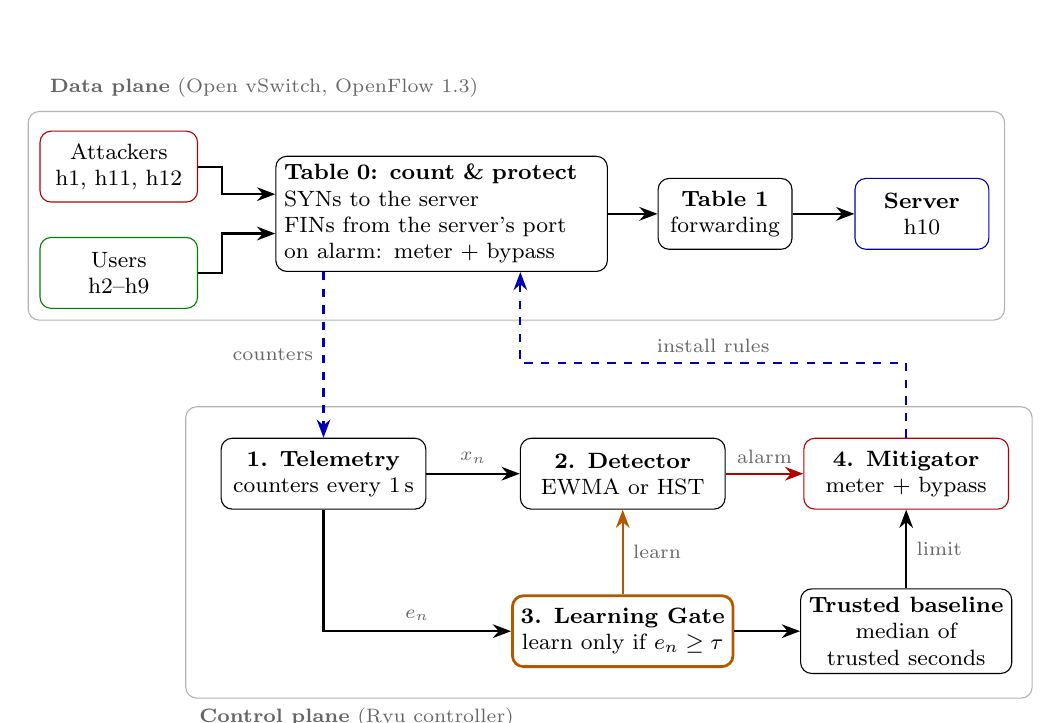
\begin{tikzpicture}[x=1cm,y=1cm,>=Stealth,
  b/.style={draw,rounded corners,align=center,font=\footnotesize,inner sep=3pt,minimum height=9mm},
  st/.style={b,minimum width=26mm},
  arr/.style={->,thick},
  ctl/.style={->,thick,dashed,blue!70!black},
  lbl/.style={font=\scriptsize,text=black!60,align=center}]
\node[b,draw=red!70!black,minimum width=20mm] (atk) at (0,0.6) {Attackers\\h1, h11, h12};
\node[b,draw=green!50!black,minimum width=20mm] (usr) at (0,-0.75) {Users\\h2--h9};
\node[b,align=left,text width=40mm] (t0) at (4.1,0) {\textbf{Table 0: count \& protect}\\SYNs to the server\\FINs from the server's port\\on alarm: meter + bypass};
\node[b,minimum width=17mm] (t1) at (7.7,0) {\textbf{Table 1}\\forwarding};
\node[b,draw=blue!70!black,minimum width=17mm] (srv) at (10.2,0) {\textbf{Server}\\h10};
\draw[arr] (atk.east) -- ++(0.3,0) |- ([yshift=2.5mm]t0.west);
\draw[arr] (usr.east) -- ++(0.3,0) |- ([yshift=-2.5mm]t0.west);
\draw[arr] (t0) -- (t1); \draw[arr] (t1) -- (srv);
\node[lbl,anchor=south west] at (-1,1.35) {\textbf{Data plane} (Open vSwitch, OpenFlow 1.3)};
\draw[black!30,rounded corners] (-1.15,-1.35) rectangle (11.25,1.3);
\node[st] (tel) at (2.6,-3.3) {\textbf{1. Telemetry}\\counters every 1\,s};
\node[st] (det) at (6.4,-3.3) {\textbf{2. Detector}\\EWMA or HST};
\node[st,draw=red!70!black] (mit) at (10.0,-3.3) {\textbf{4. Mitigator}\\meter + bypass};
\node[st,draw=orange!70!black,line width=1pt] (gate) at (6.4,-5.3) {\textbf{3. Learning Gate}\\learn only if $e_n \ge \tau$};
\node[st] (base) at (10.0,-5.3) {\textbf{Trusted baseline}\\median of\\trusted seconds};
\draw[arr] (tel) -- node[lbl,above]{$x_n$} (det);
\draw[arr,red!70!black] (det) -- node[lbl,above]{alarm} (mit);
\draw[arr] (tel.south) |- node[lbl,above,pos=0.75]{$e_n$} (gate.west);
\draw[arr,orange!70!black] (gate) -- node[lbl,right]{learn} (det);
\draw[arr] (gate) -- (base); \draw[arr] (base) -- node[lbl,right]{limit} (mit);
\node[lbl,anchor=north west] at (0.9,-6.15) {\textbf{Control plane} (Ryu controller)};
\draw[black!30,rounded corners] (0.85,-6.15) rectangle (11.6,-2.45);
\draw[ctl] (t0.south -| tel) -- node[lbl,left]{counters} (tel.north);
\draw[ctl] (mit.north) -- ++(0,0.95) -| node[lbl,above,pos=0.25]{install rules} ([xshift=10mm]t0.south);
\end{tikzpicture}\caption{Architecture of the proposed system (Evidence-Gated Learning).}\label{fig:architecture}\end{figure}
Refer to Figure~\ref{fig:architecture}: the detector receives the SYN rate $x_n$, the gate receives the completion ratio $e_n$ and decides whether the detector may learn, and an alarm from the detector triggers the mitigator, which uses the gate's trusted baseline to set its rate limit.

\section{Modules and Algorithms}
\textbf{Telemetry.} Table~0 holds counting rules that match on TCP flags (an ONF extension to OpenFlow 1.3, standard from OpenFlow 1.5, supported by Open vSwitch and Ryu): client SYNs to the server (SYN set, ACK clear), server FINs that enter the switch on the server's own port, and server SYN-ACKs. Each rule counts and then passes packets to table~1, so forwarding is unchanged. The controller requests these counters once per second and computes per-second rates. Because the FIN rule is tied to the server's port, an attacker elsewhere cannot add to it.

\textbf{Detectors.} Three lightweight detectors share one interface, \texttt{observe(rates, allow\_learning)}. \emph{Static} computes the mean and standard deviation of the SYN rate during warm-up and alarms when the z-score exceeds 3; it never adapts afterwards. \emph{EWMA} updates $\mu_{n+1} = \mu_n + \beta(x_n-\mu_n)$ and $\sigma^2_{n+1} = (1-\beta)\sigma^2_n + \beta(x_n-\mu_n)^2$, alarms when $x_n > \mu_n + \kappa\sigma_n$ ($\beta=0.1$, $\kappa=3$) and never lets $\sigma$ fall below $\sqrt{\mu}$. \emph{Half-Space Trees} \citep{tan2011hst} build 25 random trees of depth 10 over the logarithms of the SYN rate and of the packets sent to the server; a point that falls into rarely visited regions is anomalous. The reference is renewed every 20 seconds, and the alarm threshold is half of the lowest calibration score. The detectors never see $e_n$.

\textbf{Learning Gate.} The gate implements Equation~\eqref{eq:gate} with $\tau = 0.7$. It keeps the median SYN rate of the windows it approved as a \emph{trusted baseline}. Algorithm~\ref{alg:example} shows the per-second loop. In the first version, detectors learned from every warm-up second regardless of the gate, so a flood that started during warm-up was learned as normal. In the current version, a warm-up second counts only if the gate accepts it; if the gate keeps rejecting, warm-up ends after three times its normal length using the clean seconds collected (at least five).
\begin{algorithm}
\caption{Evidence-gated detection (executed every second)}\label{alg:example}
\begin{algorithmic}[1]
\Require Counters $c_n$ from table~0, detector $D$ with state $\theta$, threshold $\tau$
\Ensure Alarm $a_n$; updated state $\theta$
\State $x_n \gets$ SYN rate from $c_n - c_{n-1}$
\State $e_n \gets \sum$ FIN $/ \sum$ SYN over the last 5 s \Comment{none if fewer than 3 SYNs}
\State $a_n \gets D.\mathrm{score}(x_n;\theta)$ \Comment{no alarms while warming up}
\State $g_n \gets (e_n \text{ is none}) \lor (e_n \ge \tau)$
\If{$g_n$ \textbf{and} $e_n$ is not none}
\State add $x_n$ to the trusted baseline
\EndIf
\If{$a_n = 0$ \textbf{and} $g_n$}
\State $\theta \gets U(\theta, x_n)$ \Comment{also counts as a warm-up second}
\EndIf
\If{$a_n = 1$} \State send alarm to the mitigator \EndIf
\State \Return $a_n$
\end{algorithmic}
\end{algorithm}

\textbf{Selective mitigation.} A plain SYN rate limit mostly blocks legitimate users, because during a $10\times$ flood about nine in ten SYNs are fake. The mitigator uses the evidence again: each server FIN is also copied to the controller (only these packets), and its destination is recorded as a verified client. Algorithm~\ref{alg:mitigation} summarizes the mitigation.
\begin{algorithm}
\caption{Selective mitigation with verified-client bypass}\label{alg:mitigation}
\begin{algorithmic}[1]
\Require Alarm events, verified client set $V$, trusted baseline $b$
\State \textbf{on} alarm: install meter limiting SYNs to the server to $\max(1.5\,b,\ 5)$ per second
\ForAll{$v \in V$ verified in the last 10 minutes}
\State install a higher-priority rule so SYNs from $v$ skip the meter (still counted)
\EndFor
\State \textbf{on} new verified client while mitigating: add its bypass rule
\State \textbf{on} alarm cleared for 10 s: remove the meter and all bypass rules
\end{algorithmic}
\end{algorithm}

\section{Design Alternatives}
\begin{itemize}
\item \textbf{Packet-In versus counters.} Sending packets to the controller gives more detail, but its cost grows with the attack and is itself a known weak point of SDN. Flow counters keep the controller's work constant.
\item \textbf{Volume features versus completion evidence.} A slow attack and a legitimate crowd look the same in volume, so no volume-only detector can separate them; completion evidence differs sharply between the two.
\item \textbf{Replacing the detector versus gating it.} Using $e_n$ directly as a detector would not reuse existing detectors. Gating only what a detector learns keeps the method independent of the detector (EWMA and Half-Space Trees are both used).
\item \textbf{Drift budget.} Limiting how fast the baseline may grow also stops slow attacks, but it equally stops legitimate crowds that grow faster than the budget, so it is kept as an option, not the default.
\item \textbf{Supervised ML.} A trained classifier needs labelled SDN data and does not adapt after training; an online detector protected by the gate needs no labels.
\item \textbf{Plain meter versus bypass.} A plain meter was evaluated and harmed users more than the flood; the verified-client bypass was therefore selected.
\end{itemize}

\chapter{Implementation}
\section{Tools and Technologies}
\begin{itemize}
\item \textbf{Mininet 2.3.0} \citep{lantz2010mininet} for the emulated network.
\item \textbf{Open vSwitch} \citep{pfaff2015ovs}: version 3.3.9 with the user-space datapath (development container, Ubuntu 24.04) and the Linux kernel datapath (laptop, Ubuntu on WSL2) for the main evaluation.
\item \textbf{Ryu 4.34} \citep{ryu} as the SDN controller, using \textbf{OpenFlow 1.3} \citep{onf2012of13} (multiple tables, meters, and TCP-flag matching through the ONF extension).
\item \textbf{Python 3} for the controller applications, traffic generators and analysis; \textbf{matplotlib} for figures; \texttt{curl} for legitimate users; Linux raw sockets for the attack generator.
\item \textbf{Bash} scripts for automation, and Python \texttt{unittest} for 62 unit tests.
\end{itemize}

\section{Data and Resources}
No external dataset is used. All data is generated in the testbed by the experiments themselves: per-second telemetry, every detector's verdict, mitigation actions, every user request with its result and connect time, and the server's number of half-open connections. The detectors are unsupervised and learn online, so there is no training/test split; each detector learns during the first 60 seconds of each run (warm-up) and then keeps learning or not according to its rule. Parameter studies of $\tau$ and the drift budget replay the recorded telemetry offline, so all settings are compared on identical traffic. The main evaluation ran on a laptop (WSL2, kernel datapath); later validation runs ran in a cloud container (user-space datapath).

\section{Implementation Details}
The system is implemented as three Ryu applications and supporting modules, all of which are complete and integrated (Table~\ref{tab:modules}).
\begin{table}[htbp]\centering\caption{Implemented modules and their status}\label{tab:modules}\begin{tabularx}{\textwidth}{lXl}\toprule Module & Function & Status\\\midrule
\texttt{egl\_controller} & Two-table pipeline, counting rules, 1 s polling, completion ratio & Complete\\
\texttt{detectors} & Static, EWMA and Half-Space Trees with one interface & Complete\\
\texttt{gate} & Learning Gate, trusted baseline, optional drift budget & Complete\\
\texttt{detector\_app} & Runs all detectors with and without the gate side by side & Complete\\
\texttt{mitigator\_app} & OpenFlow meter, verified clients, bypass rules, release & Complete\\
\texttt{syn\_sender}, \texttt{http\_flood} & Abrupt/ramp spoofed SYN flood; completing bots & Complete\\
\texttt{topology}, \texttt{scenario} & 12-host topology, server, users, crowds, distributed attack & Complete\\
\texttt{run\_eval.sh}, \texttt{analyze\_eval} & Resumable evaluation; tables and figures with 95\% CI & Complete\\
\bottomrule\end{tabularx}\end{table}

\textbf{Topology.} Three switches are used: s1 and s2 are access switches connected to a central switch s3. Hosts h1--h5 and h11 connect to s1, h6--h10 to s2, and h12 to s3. The server h10 (10.0.0.10) is on port 6 of s2 and runs a threaded web server with a backlog of 511 and SYN cookies disabled. Users run on h2--h4 and h6--h9 and request a page every 0.5 seconds; in the mitigation experiments each user host uses a pool of 20 addresses and the server treats every visitor as new. The attack is split over h1, h11 and h12 on all three switches, and h5 acts as the server's gateway so replies to spoofed addresses leave the network.

\textbf{Attack generator.} A raw-socket sender produces spoofed SYNs at an exact rate every second, following an abrupt or exponential-ramp schedule ($10\times$ the users' rate, about 60 SYN/s). Tools such as \texttt{hping3} could not change rate during a run and overshot the planned rate. The switch counted 98--99\% of the planned packets.

\textbf{Integration status.} Detection and mitigation run as separate applications connected by controller events, so either can be replaced. All five detector configurations, the warm-up fix and the distributed attack are implemented and have been evaluated.

\section{Sample Code}
\begin{lstlisting}[language=Python,caption={Learning Gate decision and its use in the detector application}]
def decide(self, rates, completion):
    if completion is None:              # fewer than 3 SYNs
        return GateDecision(True, "no-traffic")
    if completion < self.tau:           # tau = 0.7
        return GateDecision(False, "low-completion")
    self._approved.append(rates["syn"]) # trusted window
    return GateDecision(True, "evidence")

# in the detector application, every second
decision = gate.decide(window.rates, window.completion)
verdict = detector.observe(window.rates,
                           allow_learning=decision.open)
if verdict.alarm:
    self.send_event_to_observers(EventAlarm(detector.name, ...))
\end{lstlisting}

\section{Reproducibility}
The code, raw results and the scripts that produce every table and figure are available at \url{https://github.com/Anirudh-N-15/mininet} (branch \texttt{egl}). Each development step has a script that starts Open vSwitch and Ryu, builds the topology, runs the scenario and checks the result:
\begin{lstlisting}[caption={Running the steps and the full evaluation}]
./egl/run_step1.sh          # telemetry and completion ratio
./egl/run_step4.sh          # detectors with the Learning Gate
./egl/run_step5.sh          # mitigation
./egl/run_eval.sh kernel    # full evaluation (resumable)
python3 -m egl.analyze_eval # tables and figures
python3 -m unittest discover egl
\end{lstlisting}

\chapter{Results and Discussion}
\section{Experimental Setup}
The main evaluation (57 runs) was carried out on a laptop running Ubuntu on WSL2 with the Open vSwitch kernel datapath. Twelve further runs, made after fixing the warm-up and distributing the attack, were carried out in a cloud container with the user-space datapath. The baselines are Static (fixed threshold, as in the earlier version of the project), EWMA and Half-Space Trees without the gate; the proposed configurations are EWMA + gate and HST + gate. All five run on the same telemetry in every run. Each run starts with 60 seconds of normal traffic from three users (about 6 SYN/s). The scenarios are: an abrupt $10\times$ flood; a slow ramp growing by 0.5, 1 or 2\% per second up to $10\times$; a legitimate flash crowd in which users grow from 3 to 15 in 60 seconds; bots that complete real HTTP requests; a flood that starts 10 seconds after the users (inside the warm-up); and the attack distributed over three hosts. Mitigation was tested with no mitigation, a plain meter, and the meter with verified-client bypass. Each case was repeated 3 to 5 times.

\section{Evaluation Metrics}
\begin{itemize}
\item \textbf{Detection rate}: runs in which an attack raised an alarm, out of all runs.
\item \textbf{Time to first alarm} after the attack started.
\item \textbf{Amplification at the first alarm}: the attack rate as a multiple of the users' normal rate. This is the main measure for slow attacks, since a slow attack is always caught eventually by a fixed detector, and what matters is how large it was allowed to grow.
\item \textbf{False alarms}: flash-crowd runs with any alarm.
\item \textbf{Requests failed or delayed}: the share of user requests that failed or needed a SYN retry (about 1 s or more extra); this measures the cost to users.
\item \textbf{Half-open peak}: the largest number of half-open connections on the server, a measure of server stress.
\end{itemize}
Results are reported as mean $\pm$ 95\% confidence interval (Student's $t$) where several runs detected the attack.

\section{Preliminary Results}
\textbf{Telemetry.} With 200 spoofed SYNs per second, the completion ratio fell from 1.000 to 0.029 (laptop: 0.030) and returned to 1.000 afterwards, matching the expected $1/m$.

\textbf{Detection.} Table~\ref{tab:detection} shows the main detection results. Every detector caught the abrupt flood in about one second. Without the gate, EWMA and Half-Space Trees learned the slow ramp: EWMA caught it in 1 of 5 runs and only at $10.2\times$ (the single HST detection was an alarm on a brief traffic dip). Static caught the ramp but raised a false alarm on every flash crowd. EWMA + gate was the only configuration that caught the slow attack in every run while staying quiet on crowds; its one crowd false alarm occurs in the same run with and without the gate.
\begin{table}[htbp]\centering\caption{Detection results (5 runs per scenario, ramp +0.5\%/s)}\label{tab:detection}\begin{tabular}{lccc}\toprule Detector & Abrupt $10\times$ & Slow ramp (amplification) & Crowd false alarms\\\midrule
Static & 5/5 (1.1 s) & 5/5 ($2.17\pm0.11\times$) & 5/5\\
EWMA & 5/5 (1.1 s) & 1/5 ($10.21\times$) & 1/5\\
Half-Space Trees & 5/5 (1.1 s) & 1/5 & 5/5\\
\textbf{EWMA + gate} & \textbf{5/5 (1.1 s)} & \textbf{5/5 ($2.89\pm0.11\times$)} & \textbf{1/5}\\
HST + gate & 5/5 (1.1 s) & 5/5 ($1.93\pm1.02\times$) & 5/5\\\bottomrule\end{tabular}\end{table}

The gate closed at $1.43\times$ the normal rate, as predicted by $1/m < \tau$. With the baseline frozen there, the predicted alarm level was about $2.9\times$, and the measured value was $2.89\pm0.11\times$. Table~\ref{tab:growth} shows that this holds for faster ramps.
\begin{table}[htbp]\centering\caption{Detection at different ramp speeds (detected, amplification at alarm)}\label{tab:growth}\begin{tabular}{lccc}\toprule Detector & +0.5\%/s (5 runs) & +1\%/s (3 runs) & +2\%/s (3 runs)\\\midrule
Static & 5/5 ($2.17\times$) & 3/3 ($2.25\times$) & 3/3 ($2.19\times$)\\
EWMA & 1/5 ($10.21\times$) & 1/3 ($15.23\times$) & 0/3\\
Half-Space Trees & 1/5 & 2/3 ($3.27\times$) & 3/3 ($5.04\times$)\\
\textbf{EWMA + gate} & \textbf{5/5 ($2.89\times$)} & \textbf{3/3 ($2.83\times$)} & \textbf{3/3 ($2.72\times$)}\\
HST + gate & 5/5 ($1.93\times$) & 3/3 ($1.96\times$) & 3/3 ($2.54\times$)\\\bottomrule\end{tabular}\end{table}

\textbf{Attack during warm-up and distributed attack.} Table~\ref{tab:early} compares the first version of the gate with the fixed warm-up on a flood starting 10 seconds after the users, and summarizes the distributed attack. Replaying all 48 earlier gated results with the fixed code gives the same answers, so the fix does not change the other results.
\begin{table}[htbp]\centering\caption{Attack during warm-up (3 runs) and distributed attack (9 runs)}\label{tab:early}\begin{tabularx}{\textwidth}{Xl}\toprule Case & Result\\\midrule
Flood in warm-up: Static, EWMA, HST & 0/3 detected\\
Flood in warm-up: EWMA + gate and HST + gate, first version & 0/3 detected\\
\textbf{Flood in warm-up: EWMA + gate and HST + gate, fixed} & \textbf{3/3 detected (49 s after start)}\\
Distributed abrupt flood (3 hosts): every detector & 2/2, about 1 s\\
Distributed ramp +1\%/s: EWMA + gate / plain EWMA & 2/2 at $3.09\times$ / 0/2\\
Distributed, bypass mitigation: requests failed or delayed & 0.7\% (none: 20.6\%)\\
\bottomrule\end{tabularx}\end{table}

\textbf{Mitigation.} Table~\ref{tab:mitigation} shows the effect on users and on the server (3 runs each). Without mitigation the half-open queue filled (385 entries, where Linux starts refusing new SYNs) and about a third of requests were delayed. The plain meter made things worse for users. With the verified-client bypass, only 0.4\% of requests were affected; with either meter the queue levelled off at about 258, just above half full, where Linux starts removing old half-open entries early. During a flash crowd, a false alarm from Static with a plain meter affected a quarter of requests, while the bypass kept every user unaffected. Varying the meter limit from 0.5 to 2.5 times the trusted baseline changed the affected requests only between 1.1\% and 1.4\%.
\begin{table}[htbp]\centering\caption{Effect of mitigation (requests failed or delayed; half-open peak)}\label{tab:mitigation}\begin{tabular}{lccc}\toprule Scenario & No mitigation & Plain meter & Meter + bypass\\\midrule
Abrupt $10\times$ (EWMA + gate) & 34.5\%; 385 & 87.7\%; 257 & \textbf{0.4\%; 258}\\
Ramp +1\%/s (EWMA + gate) & 2.9\%; 385 & 21.1\%; 258 & \textbf{0.0\%; 258}\\
Flash crowd (Static false alarm) & 0.0\%; 0 & 25.8\%; 0 & \textbf{0.0\%; 1}\\\bottomrule\end{tabular}\end{table}

\section{Qualitative Results}
Figure~\ref{fig:frog} shows the problem: the same $10\times$ flood is caught at once when it is abrupt, and never when it ramps. Figure~\ref{fig:detectors} shows one run of each scenario for all detectors, with the seconds in which the gate was closed. Figure~\ref{fig:results} follows one abrupt flood second by second, with and without mitigation, and Figure~\ref{fig:mitigationbars} summarizes the mitigation over repeated runs. Figure~\ref{fig:tau} shows the effect of $\tau$: a higher threshold catches the ramp earlier ($5.65\times$ at $\tau = 0.3$, $2.34\times$ at $0.95$), while false alarms on crowds do not change.
\begin{figure}[htbp]
\centering
\IfFileExists{figures/step2_ramp_vs_abrupt.png}{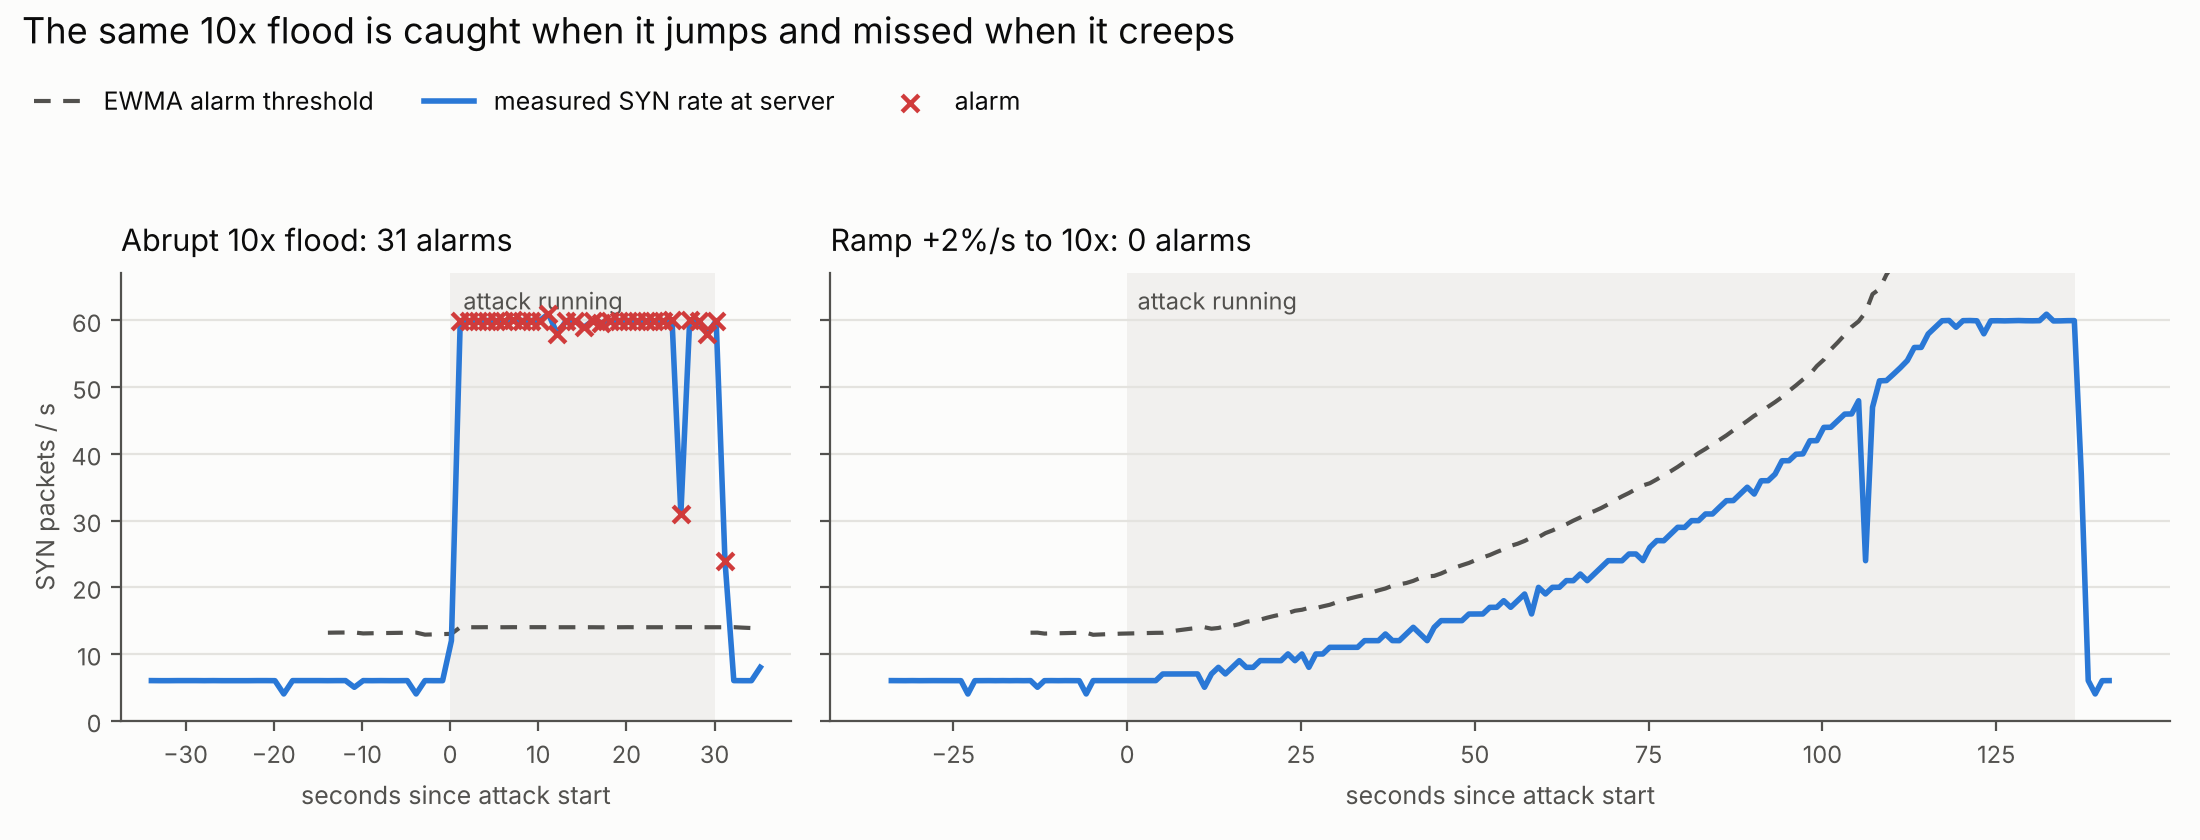
\includegraphics[width=\linewidth]{figures/step2_ramp_vs_abrupt.png}}{\fbox{\parbox[c][35mm][c]{.75\linewidth}{\centering Replace with actual experimental figure}}}
\caption{The same $10\times$ SYN flood, abrupt and as a slow ramp, against EWMA}\label{fig:frog}
\end{figure}
\begin{figure}[htbp]
\centering
\IfFileExists{figures/step4_detectors.png}{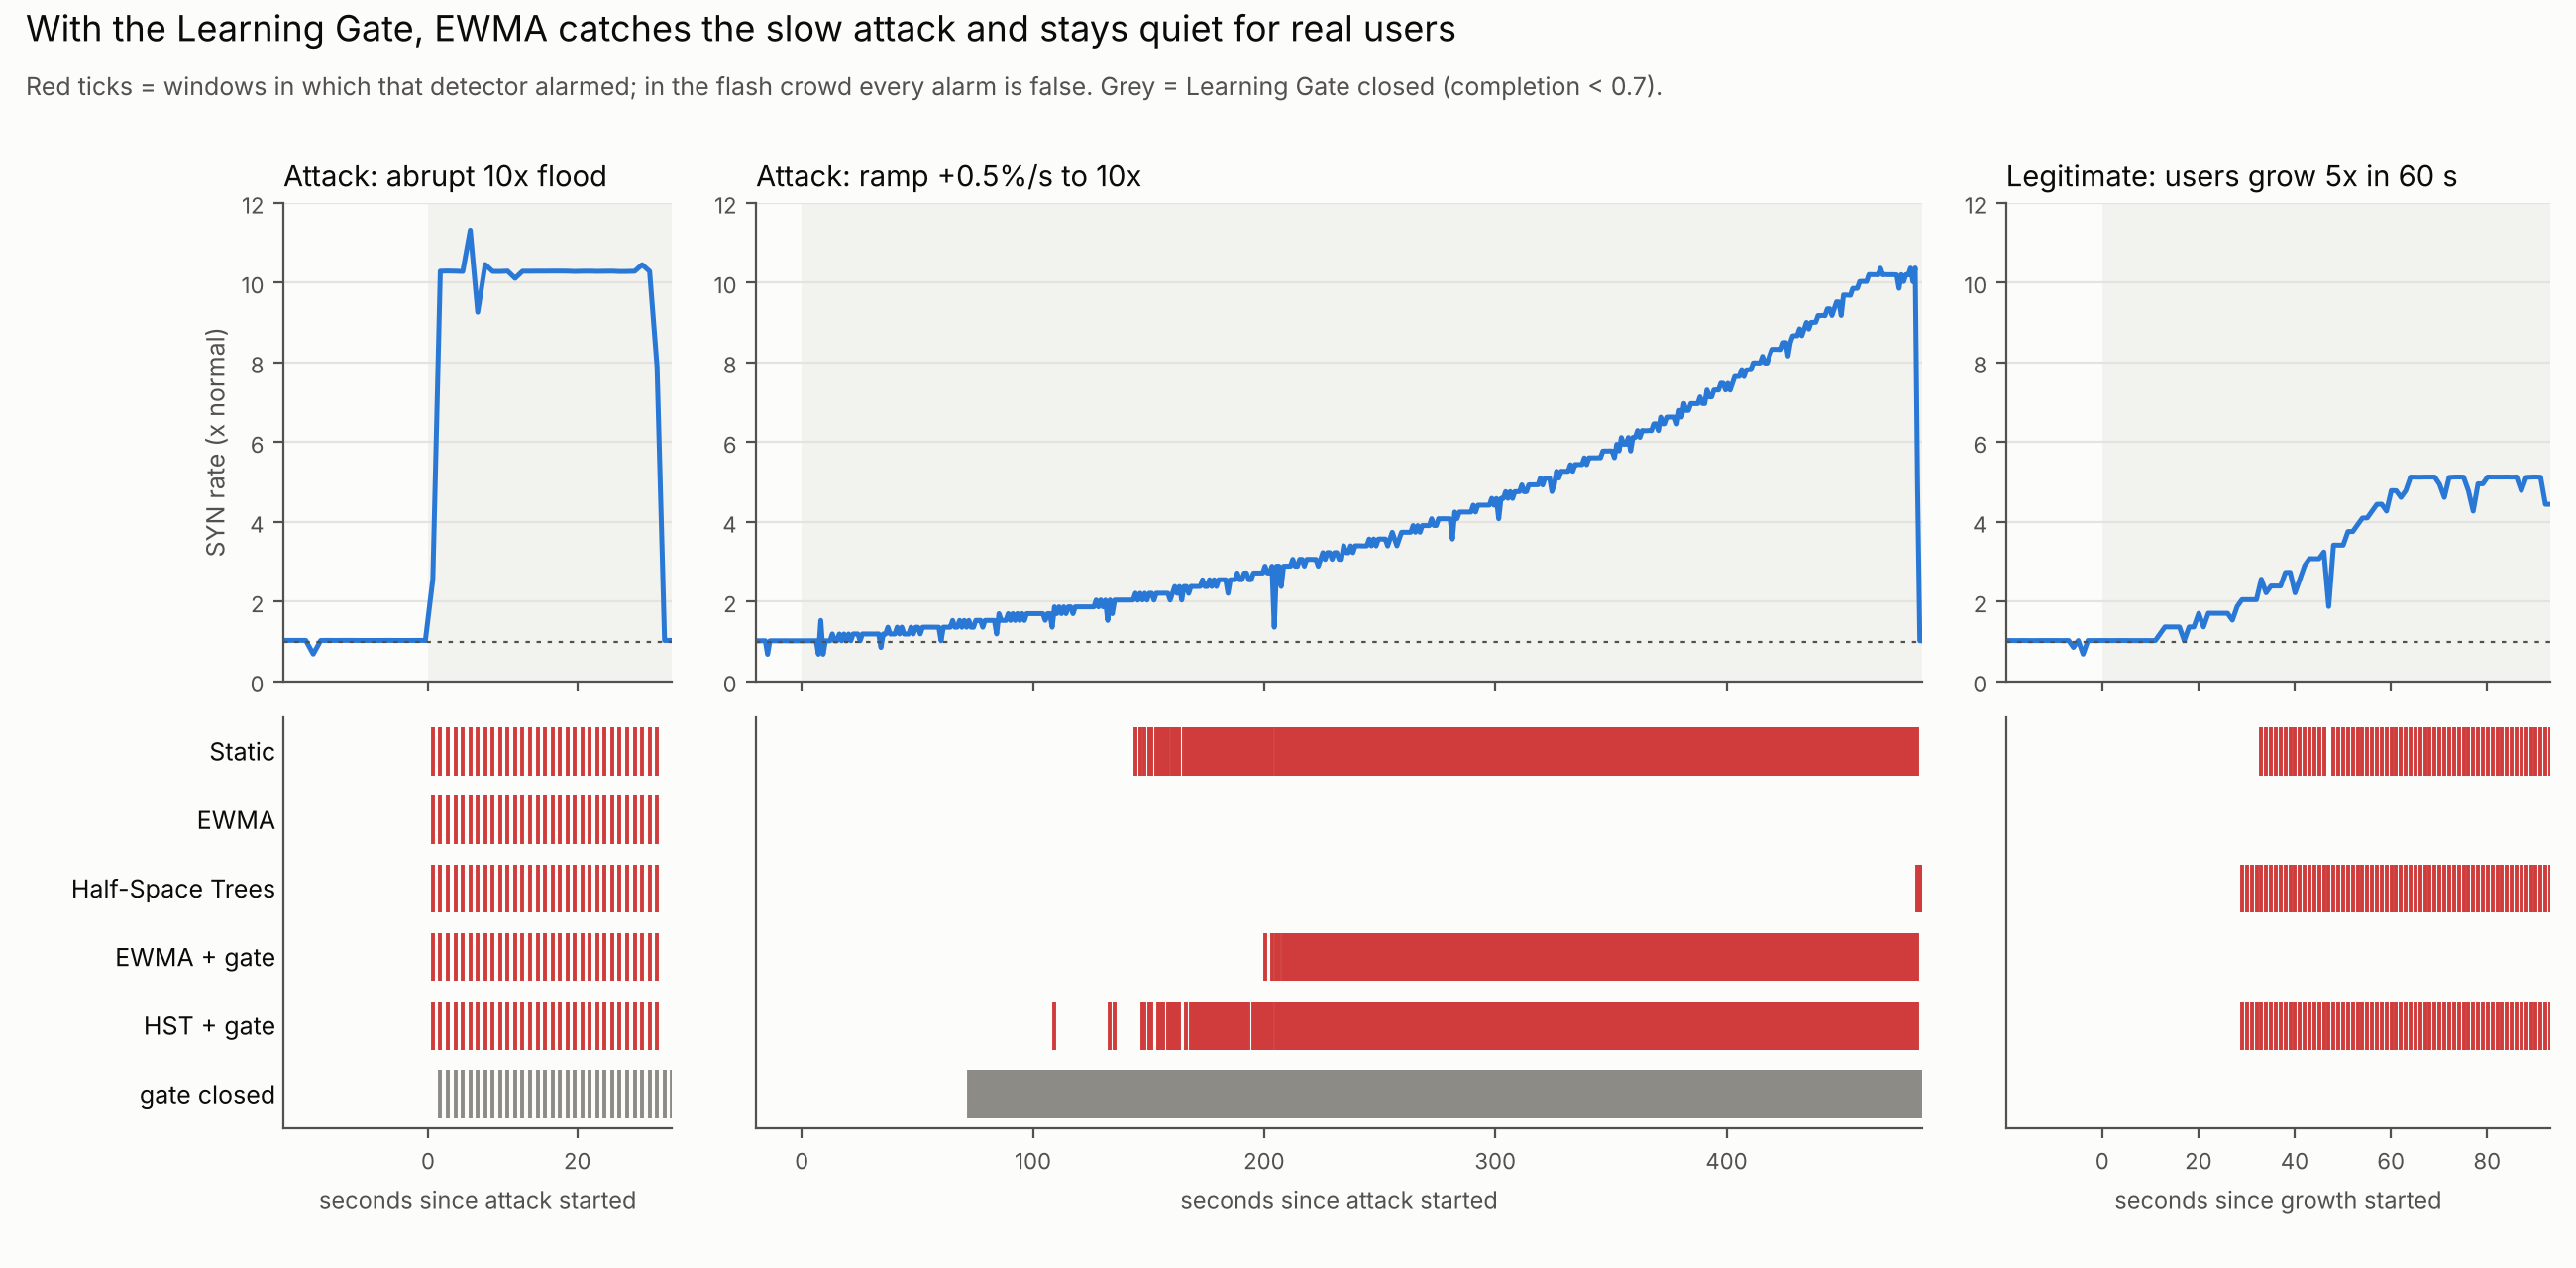
\includegraphics[width=\linewidth]{figures/step4_detectors.png}}{\fbox{\parbox[c][35mm][c]{.75\linewidth}{\centering Replace with actual experimental figure}}}
\caption{Alarms of all detectors on the abrupt flood, slow ramp and flash crowd}\label{fig:detectors}
\end{figure}
\begin{figure}[htbp]
\centering
\IfFileExists{figures/fig_timeline_abrupt.png}{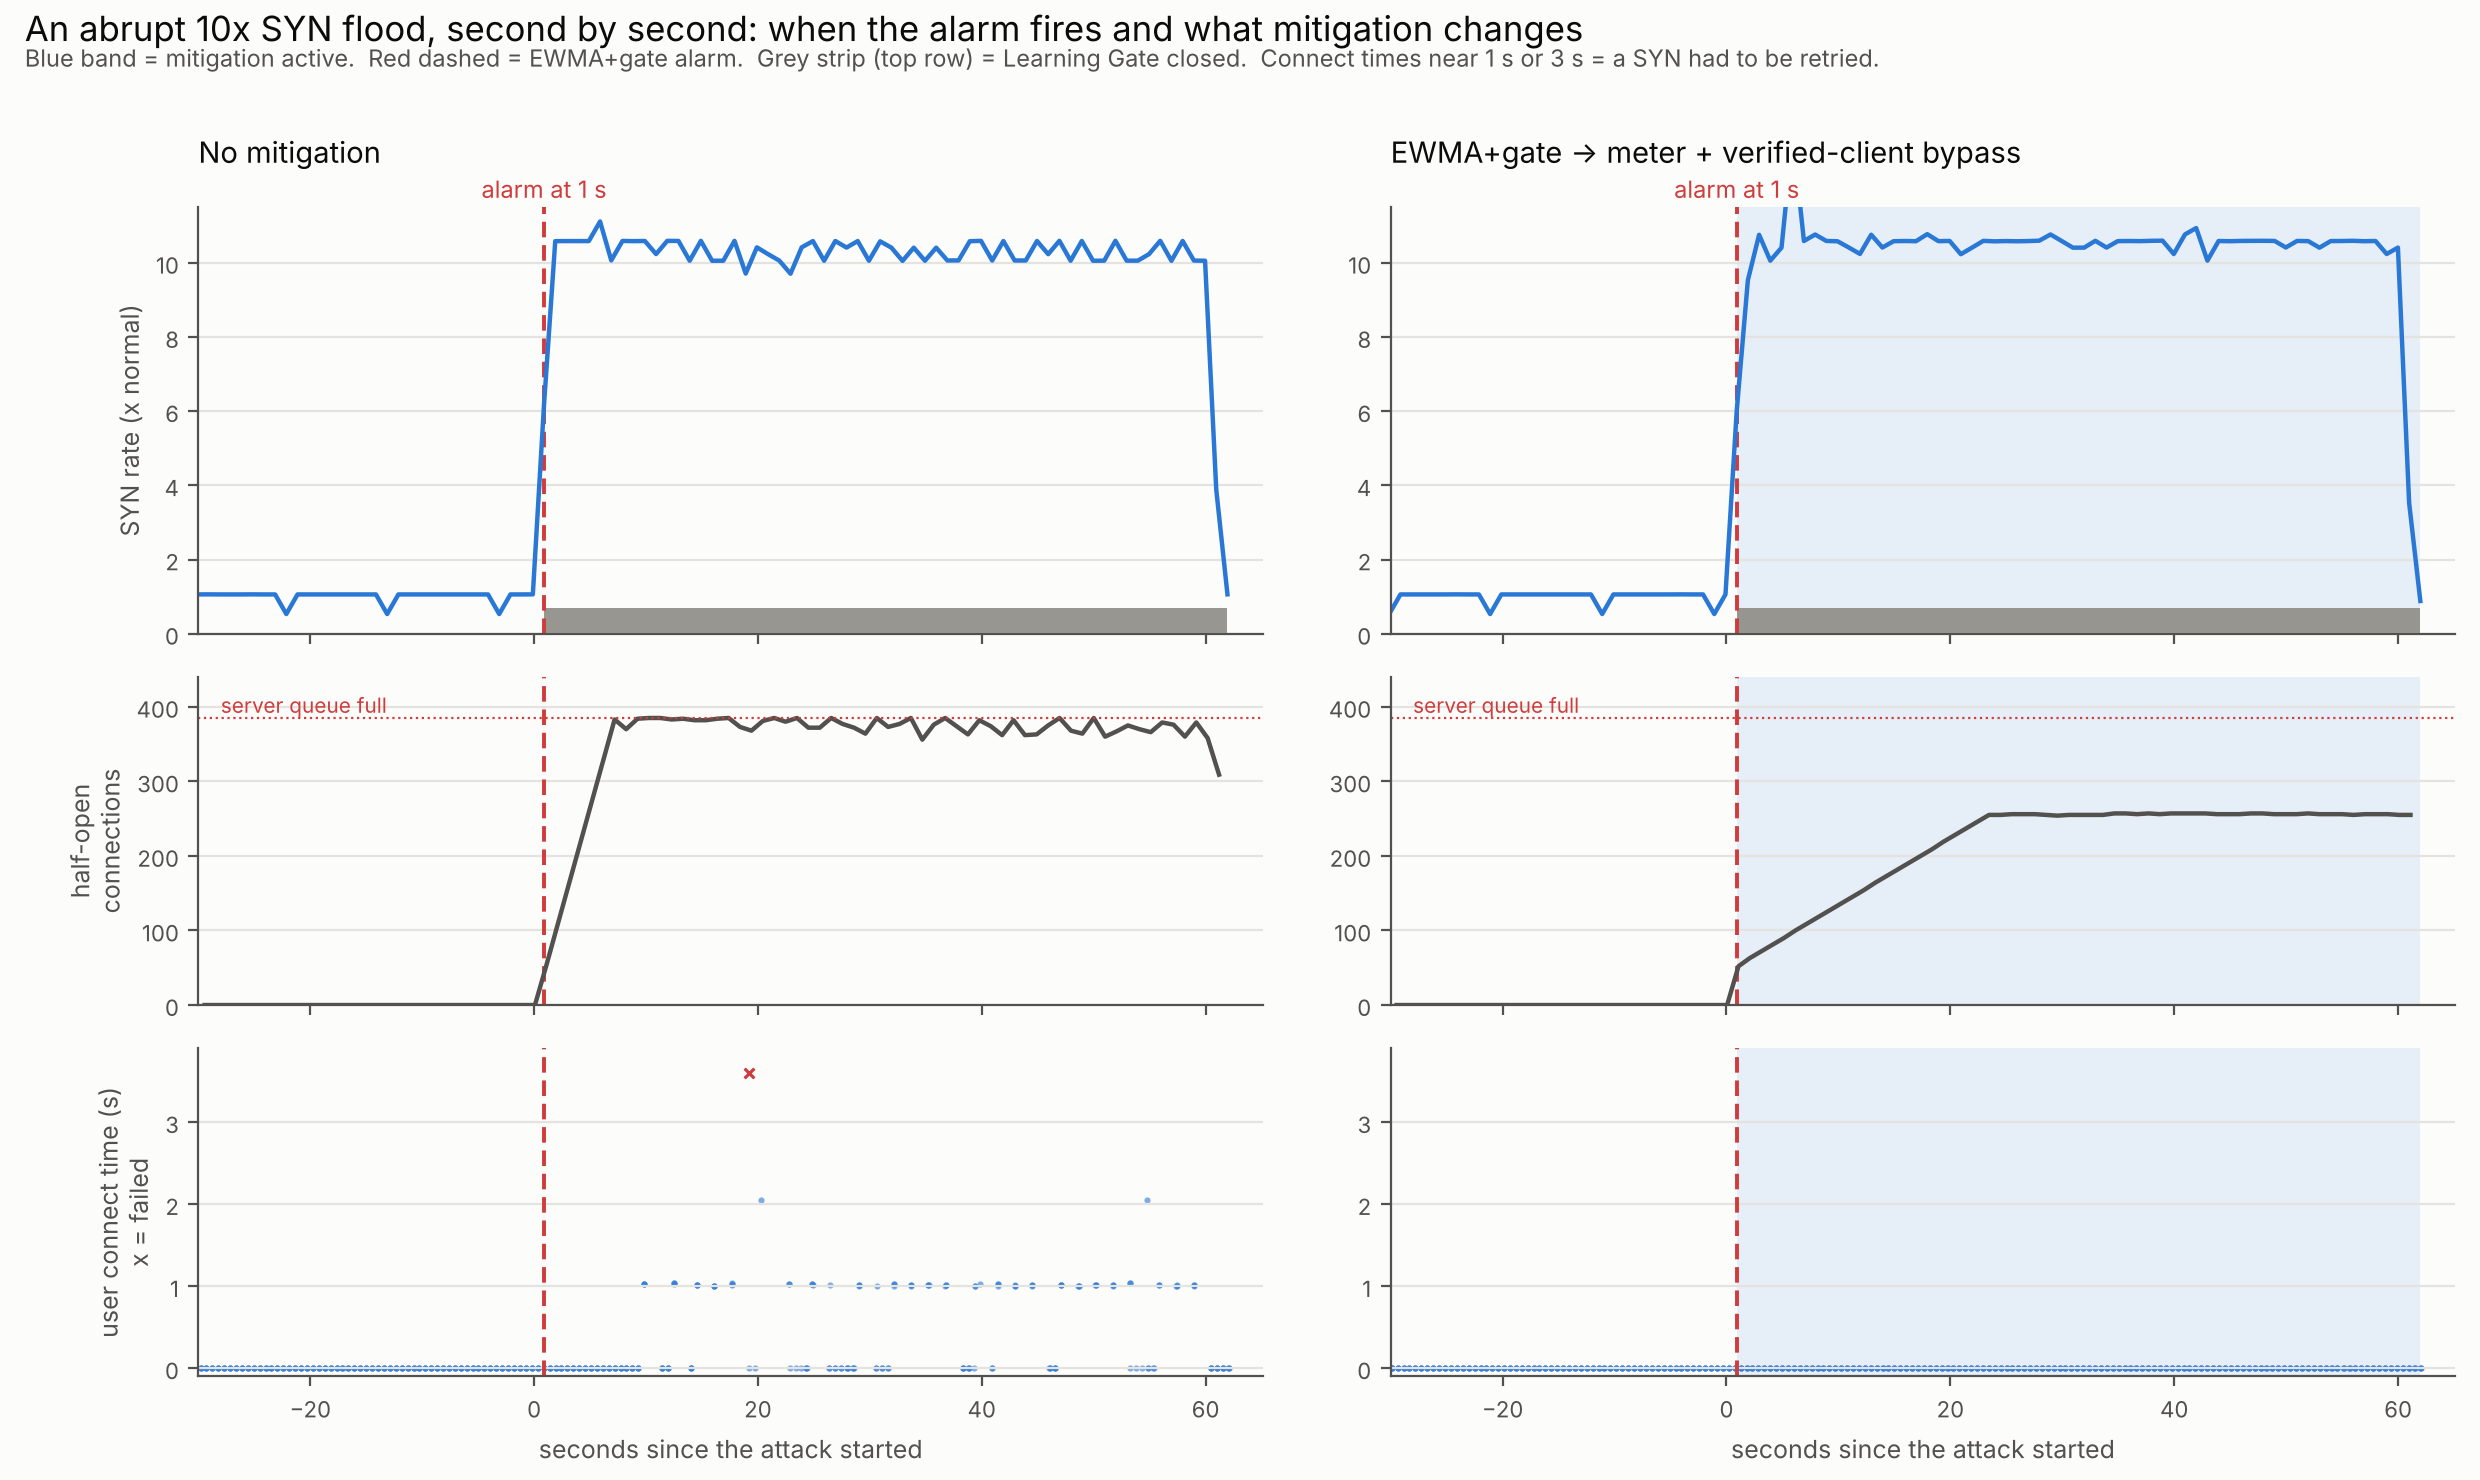
\includegraphics[width=\linewidth]{figures/fig_timeline_abrupt.png}}{\fbox{\parbox[c][35mm][c]{.75\linewidth}{\centering Replace with actual experimental figure}}}
\caption{Abrupt flood second by second, without mitigation and with meter + bypass}\label{fig:results}
\end{figure}
\begin{figure}[htbp]
\centering
\IfFileExists{figures/fig_mitigation.png}{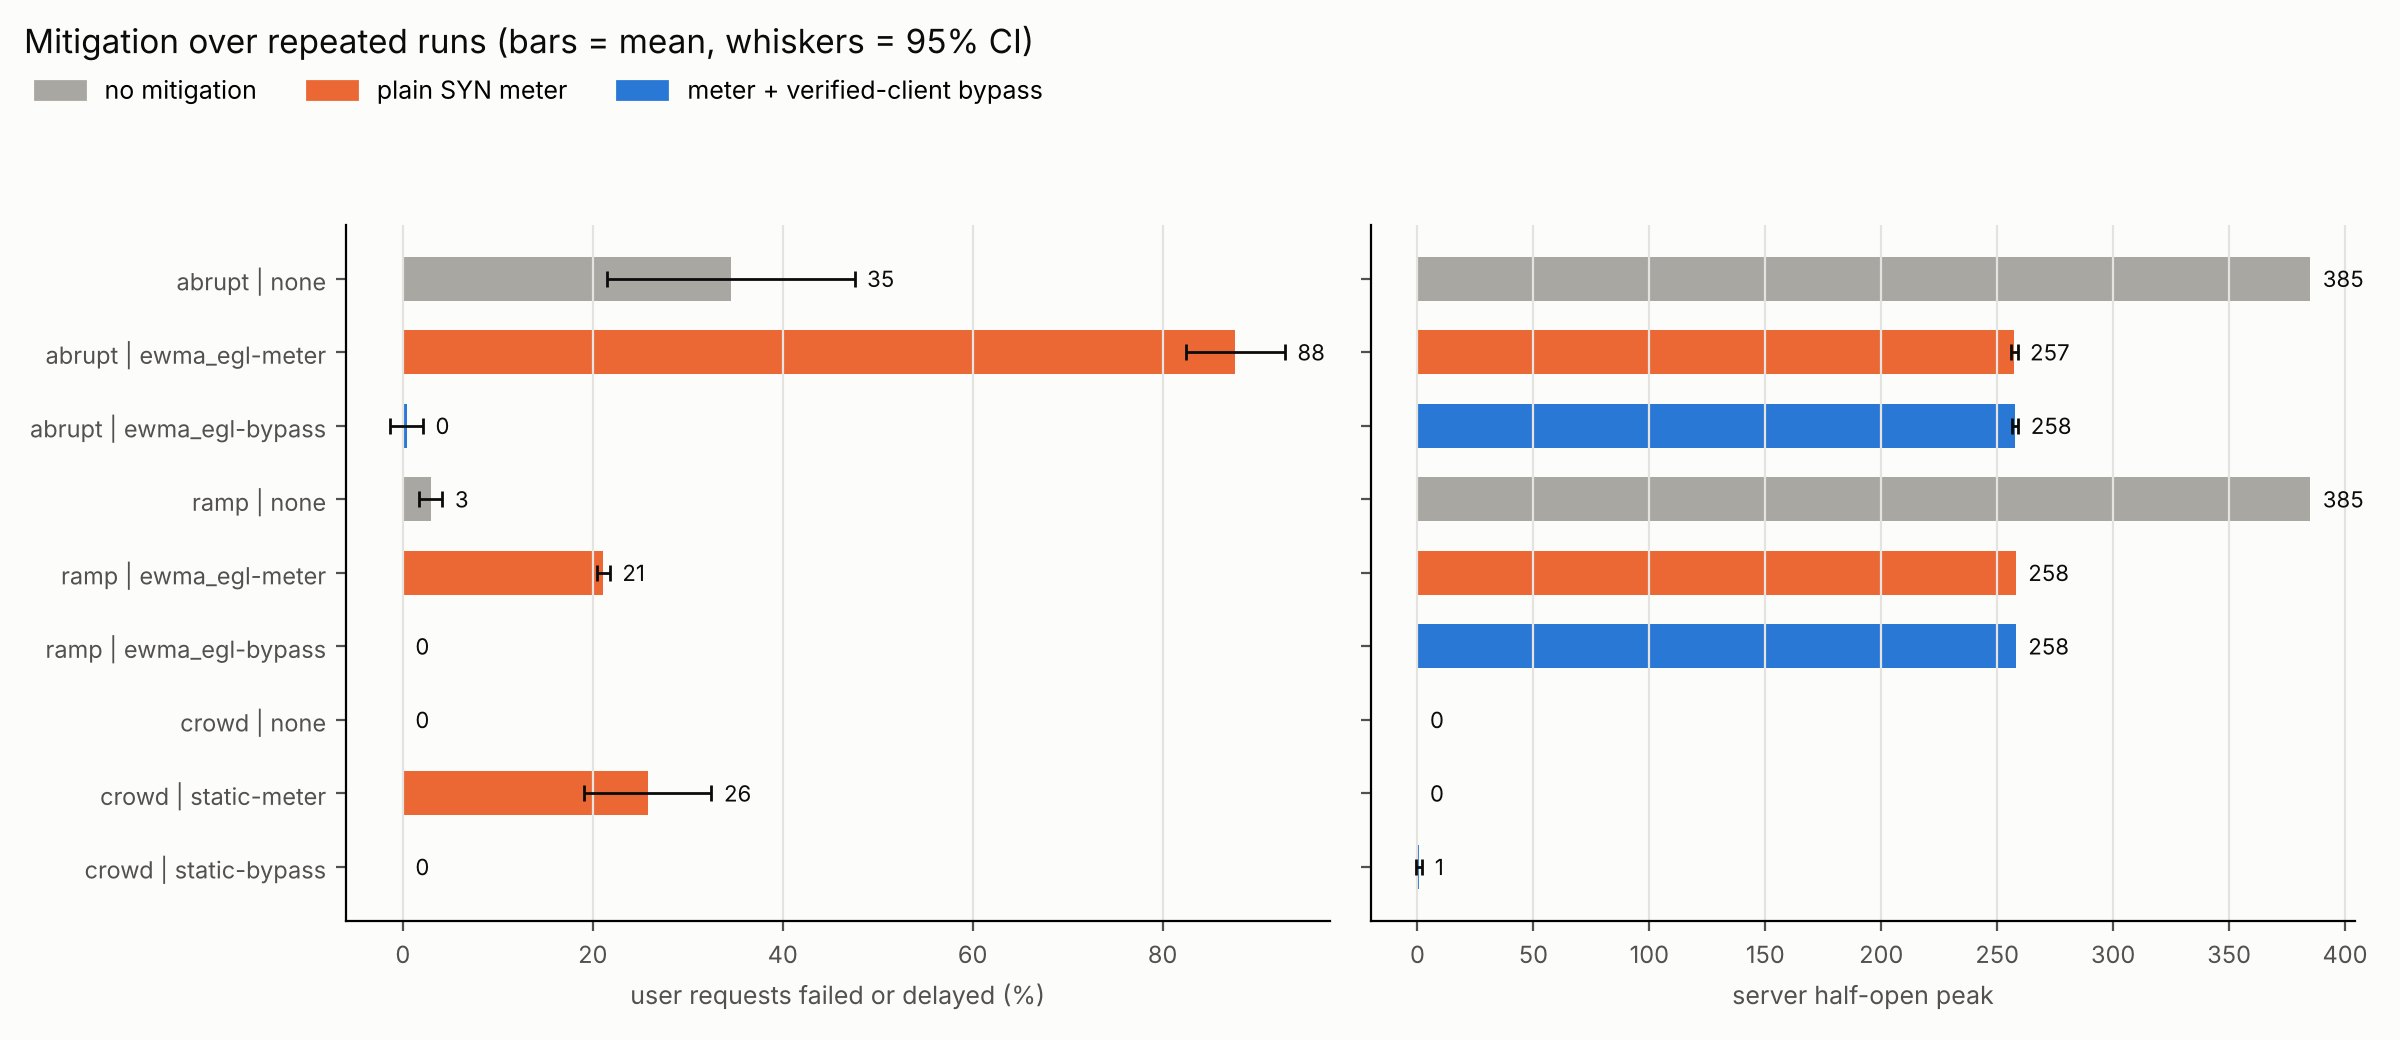
\includegraphics[width=\linewidth]{figures/fig_mitigation.png}}{\fbox{\parbox[c][35mm][c]{.75\linewidth}{\centering Replace with actual experimental figure}}}
\caption{Requests failed or delayed, and half-open peak, under each mitigation policy}\label{fig:mitigationbars}
\end{figure}
\begin{figure}[htbp]
\centering
\IfFileExists{figures/fig_tau.png}{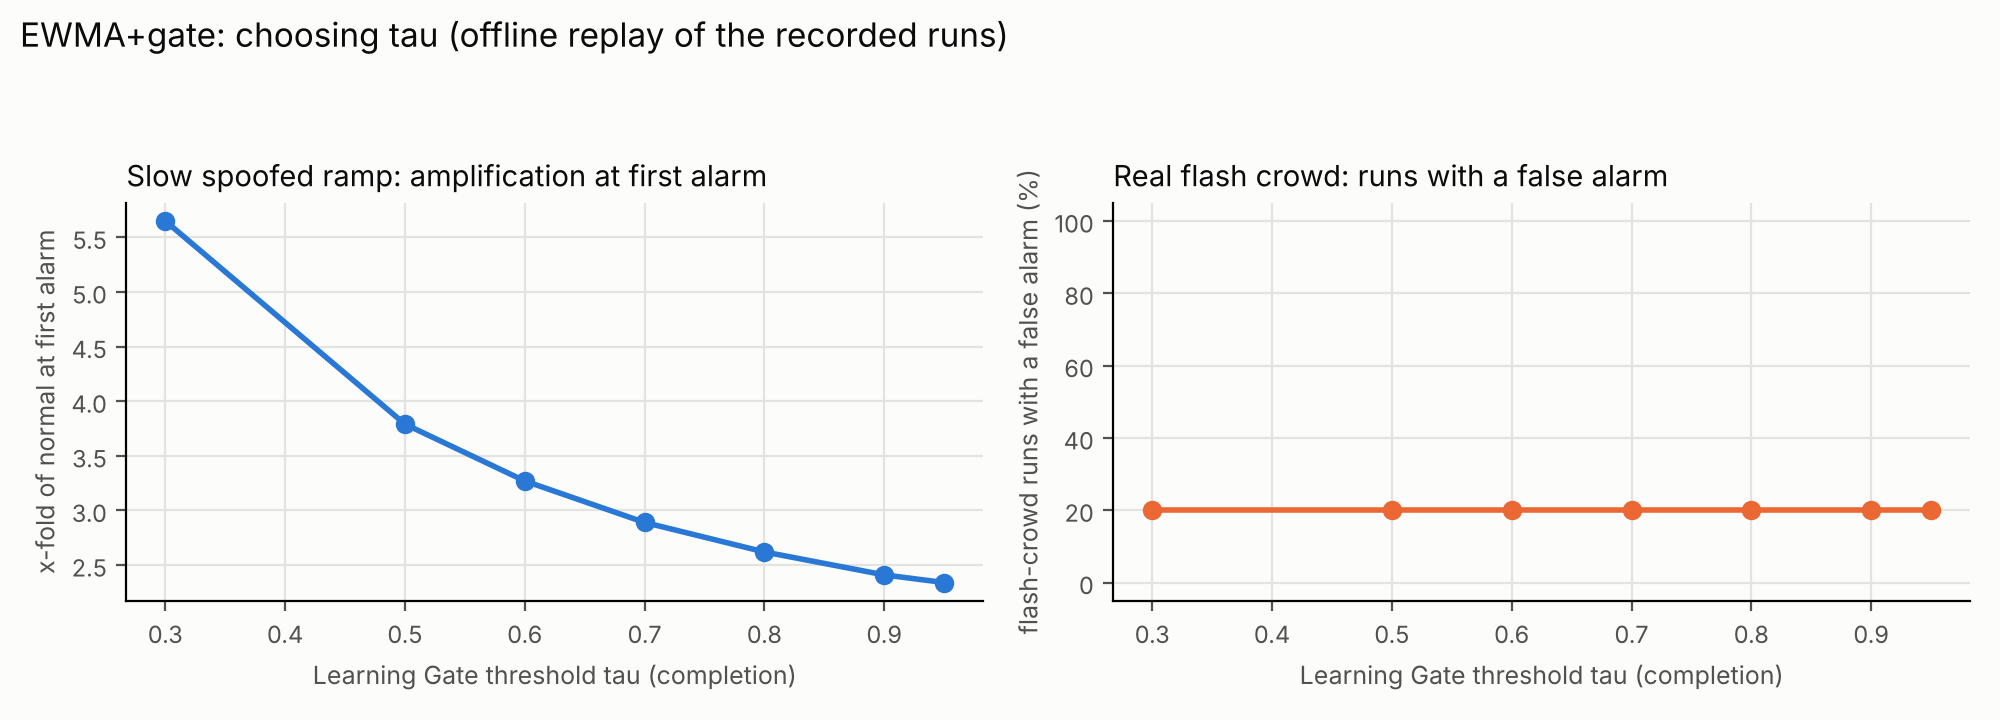
\includegraphics[width=\linewidth]{figures/fig_tau.png}}{\fbox{\parbox[c][35mm][c]{.75\linewidth}{\centering Replace with actual experimental figure}}}
\caption{Effect of the gate threshold $\tau$ (offline replay of the recorded runs)}\label{fig:tau}
\end{figure}

\section{Discussion and Limitations}
The results confirm that adaptive SDN detectors can be slowly poisoned, and that the completion ratio separates a slow attack from legitimate growth where volume alone cannot. Gating what the detector learns caught every slow attack with EWMA while legitimate crowds were still accepted, and the measured detection level matched the simple model. The same evidence made mitigation safe for users: the plain meter, the usual response, hurt more users than the flood itself.

The work also has clear limitations:
\begin{itemize}
\item \textbf{Completing bots.} Bots that use real addresses and complete real HTTP requests keep the completion ratio high, so EWMA + gate missed them in 3 of 3 runs. A drift budget of 2\% per second or less detects them (3/3), but then raises a false alarm on every legitimate flash crowd (5/5); this is a trade-off, not a fix.
\item \textbf{Alarm rule.} The gate controls what a detector learns, not how it raises alarms, so Half-Space Trees still raises false alarms on crowds with the gate.
\item \textbf{New visitors.} Clients that have never completed a connection must pass the meter during an attack before they are verified.
\item \textbf{Warm-up.} The first version did not gate the warm-up; this has been fixed, but a flood present from the very start delays detection until the extended warm-up ends (49 s in our runs).
\item \textbf{Scale and environment.} The testbed is small, with one controller and one server, and the early-attack and distributed runs used the user-space datapath with fewer repeats. Controller overhead (CPU, messages per second) has not yet been measured.
\item \textbf{Protocol.} The evidence is specific to TCP.
\end{itemize}

\chapter{Conclusion and Future Work}
\section{Summary and Contributions}
This project studied DDoS detection and mitigation in SDN, and identified and addressed a weakness of adaptive detectors. Against the objectives of Chapter~1:
\begin{enumerate}
\item \textbf{Vulnerability demonstrated.} A slowly increasing $10\times$ SYN flood went undetected by EWMA: across three ramp speeds EWMA caught the slow attack in only 2 of 11 runs, and only above $10\times$. Half-Space Trees missed the slowest ramp in 4 of 5 runs. A closed-form bound (Equation~\eqref{eq:objective}) describes how fast the attack works.
\item \textbf{Learning Gate designed and validated.} Evidence-Gated Learning, which lets a detector learn only while the server completes connections, caught the slow attack in every run (EWMA + gate: 11/11 across three ramp speeds) with no added false alarms on flash crowds, and caught floods that start during warm-up after the warm-up fix.
\item \textbf{Constant monitoring overhead.} Telemetry uses OpenFlow 1.3 flag-matching counters polled once per second, with no Packet-In messages.
\item \textbf{Selective mitigation.} Verified-client bypass reduced failed or delayed requests during a $10\times$ flood from 34.5\% to 0.4\%, where a plain meter increased them to 87.7\%.
\item \textbf{Evaluation.} 69 live runs with repeated measurements, confidence intervals and offline parameter studies; results held when the attack was distributed over three hosts.
\end{enumerate}
The main contributions are the first study, to our knowledge, of frog-boiling attacks on SDN DDoS detectors; Evidence-Gated Learning, a detector-independent defence based on unforgeable completion evidence from switch counters; and a selective mitigation that uses the same evidence to protect legitimate users.

\section{Remaining Work and Semester Eight Plan}
\begin{table}[htbp]\centering\caption{Proposed completion plan}\begin{tabularx}{\textwidth}{Xll}\toprule Task & Target date & Status\\\midrule
Re-run the early-attack and distributed experiments on the kernel datapath with full repeats & January 2027 & Planned\\
Measure controller overhead (CPU, OpenFlow messages per second) & January 2027 & Planned\\
Larger topology: more switches, users and servers; longer, varying traffic & February 2027 & Planned\\
Extend the evidence beyond SYN/FIN (RST, persistent HTTP, UDP/QUIC) & February 2027 & Planned\\
Defence against completing bots and adaptive attackers that target the gate & March 2027 & Planned\\
Write and submit a research paper (IEEE conference format) & March--April 2027 & Planned\\
Final report and presentation & April 2027 & Planned\\
\bottomrule\end{tabularx}\end{table}

\section{Individual Contributions}
This is an individual project; all the work was carried out by the student.
\begin{table}[htbp]\centering\caption{Individual contributions}\begin{tabularx}{\textwidth}{lX}\toprule Student & Contribution\\\midrule Anirudh Nambiar (B230629CS) & Literature survey; problem formulation and system design; implementation of the telemetry, detectors, Learning Gate, mitigation, traffic and attack generators and evaluation scripts; running and analysing all experiments; report and presentation.\\\bottomrule\end{tabularx}\end{table}
\clearpage
\addcontentsline{toc}{chapter}{References}
\bibliographystyle{IEEEtran}
\bibliography{references}
\appendix
\chapter{Supplementary Material}
\textbf{Evaluation stages.} The full evaluation is run by \texttt{run\_eval.sh} in the stages of Table~\ref{tab:stages}.
\begin{table}[htbp]\centering\caption{Stages of the evaluation}\label{tab:stages}\begin{tabularx}{\textwidth}{lXc}\toprule Stage & What it measures & Runs\\\midrule
detection & 5 detectors on abrupt flood, flash crowd and ramp (+0.5\%/s) & 15\\
growth & ramp at +1\%/s and +2\%/s & 6\\
completing & bots completing real HTTP requests (limitation) & 3\\
mitigation & no mitigation, plain meter, meter + bypass & 27\\
margin & meter limit 0.5, 1.0 and 2.5 times the trusted baseline & 6\\
early & flood during warm-up: first version vs fixed gate & 3\\
distributed & attack split over three hosts & 9\\\bottomrule\end{tabularx}\end{table}

\textbf{Gate threshold and drift budget.} Table~\ref{tab:ablation} gives the offline replay results for EWMA + gate.
\begin{table}[htbp]\centering\caption{Offline replay: threshold $\tau$ and drift budget $\delta$ (EWMA + gate)}\label{tab:ablation}\begin{tabular}{lccc}\toprule Setting & Ramp detected (amplification) & Completing bots & Crowd false alarms\\\midrule
$\tau = 0.3$ & 5/5 ($5.65\times$) & 0/3 & 1/5\\
$\tau = 0.5$ & 5/5 ($3.79\times$) & 0/3 & 1/5\\
$\tau = 0.7$ (default) & 5/5 ($2.89\times$) & 0/3 & 1/5\\
$\tau = 0.9$ & 5/5 ($2.41\times$) & 0/3 & 1/5\\
$\tau = 0.7$, $\delta = 2\%$/s & 5/5 ($2.89\times$) & 3/3 ($4.50\times$) & 5/5\\
$\tau = 0.7$, $\delta = 0.5\%$/s & 5/5 ($2.55\times$) & 3/3 ($2.25\times$) & 5/5\\\bottomrule\end{tabular}\end{table}

\textbf{Development milestones.} Step 1 built the two-table pipeline and counter telemetry; step 2 built the ramp attacker and demonstrated frog-boiling; step 3 added the three detectors; step 4 added the Learning Gate; step 5 added the selective mitigation and the full evaluation; a final step gated the warm-up and distributed the attack. 62 unit tests cover the counters, detectors, gate, attack schedule and metrics.
\end{document}
